\documentclass[12pt]{article}
\usepackage{url}
\usepackage{setspace}
\usepackage{graphics}
\usepackage[superscript]{cite}
\usepackage{graphicx}
\usepackage[normalem]{ulem}
\graphicspath{ {Figures/} }
\usepackage{caption}
\usepackage{cite}
\usepackage{indentfirst}
\usepackage{float}
\usepackage{subcaption}
\usepackage{amsmath}
\textwidth=6.5in
\oddsidemargin=0.0in
\usepackage{listings}
\usepackage{listings}
\usepackage{fancyhdr}
\usepackage{longtable}
\usepackage[table]{xcolor} \pagestyle{fancy} \fancyhf{}
\lhead{Strengthy}
\rhead{Page \thepage}

\usepackage{color}
\usepackage{hyperref}
\hypersetup{
    colorlinks=true,
    citecolor=black,
    linktoc=all,
    linkcolor=black,
}

\begin{document}

\begin{titlepage}

\newcommand{\HRule}{\rule{\linewidth}{0.5mm}}

\center

\textsc{\LARGE Missouri State University\\~\\Department computer Science}\\[1.0cm]

\HRule \\[0.4cm]
{ \huge \bfseries Strengthy}\\[0.4cm]
{ \large A fitness tracking webapp}\\[0.4cm]
\HRule \\[1.5cm]

\begin{minipage}{0.4\textwidth}
\begin{flushleft} \large
Dylan Bolger \\ Hayden Pope
\end{flushleft}
\end{minipage}
~
\begin{minipage}{0.4\textwidth}
\begin{flushright} \large
Client Info \\
Dr. Mohammed Y. Belkhouche\\

\end{flushright}
\end{minipage}\\[2cm]

{\large \today}\\[2cm]

\end{titlepage}

\newpage
%-----------------------------------------------------------------------
\tableofcontents

\newpage
%----------------------------------------------------------------------

%-----------------------------------------------------------------------------
\section{Project Description}
\subsection{Proposal}
Our proposal is to develop a web application to track weightlifting sessions, progress, and statistics. This web-app will allow users to create personal accounts to track their information. We will allow the user to upload their data from days at the gym and be able to watch their progress as they continue to go to the gym. It will also show useful calculations, such as percentages of your 1RM (One repetition max). Statistics like progress prediction of the user and analysis will be included. Users will also be able to create their own workout plans, or routines. The routines will suggest values in order for the user to make meaningful progression at the gym. Users can also record their weight.

\subsection{Stack}
The web application will be developed in Python using the Flask framework. A database will be used to store user information, likely SQLite. Graphs displayed to the user will be rendered using chart.js.


%-----------------------------------------------------------------------------
\section{Functional Requirements}

\subsection{Req. 1 - User Account Registration}
\begin{description}
	\item[Description] Users will be able to create there own account using an username, email, and password. The username and email must be unique, and the email must be a valid email address.
	\item[Rational] Users need to be able to create accounts to store their personal data
	\item[Inputs] Username, email, and password combo created by users
	\item[Outputs] Username, email, and password hash will be stored in a database.
	\item[Dependencies] None
\end{description}

\subsection{Req. 2 - User Account Login}
\begin{description}
	\item[Description] Users will be able to login to their account using their username and password. If the username or password are invalid, an error will be displayed to the user. Users will remained logged in using cookies to try and minimize the amount of times a user has to login during a workout session.
	\item[Rational] Users need to be able to login to their accounts to input data.
	\item[Inputs] Username and password combo provided by user.
	\item[Outputs] A cookie will be set marking the user as logged in.
	\item[Dependencies] None
\end{description}

\subsection{Req. 3 - User Account Update}
\begin{description}
	\item[Description] Users will be able to change their password.
	\item[Rational] Allow users to use whichever password they want.
	\item[Inputs] User inputs old and new password in a form.
	\item[Outputs] User's password is updated in the database.
	\item[Dependencies] User will need to be logged in.
\end{description}

\subsection{Req. 4 - User Account Deletion}
\begin{description}
	\item[Description] Users will be able to delete their account and all data attached to their account.
	\item[Rational] Users can choose not to have their data stored by Strengthy.
	\item[Inputs] User presses a delete button with a "Are you sure?" confirmation.
	\item[Outputs] User account data is deleted from the database.
	\item[Dependencies] User will need to be logged in.
\end{description}

\subsection{Req. 5 - Homepage}
\begin{description}
	\item[Description] Users will land on a homepage that outlines what Strengthy is all about. This will show images of fitness, and a bold description of what the application can do. This is expected to be efficient and speedy for users to enter on both desktop and on the mobile device.
	\item[Rational] New users need to learn what the application is, and why they might be interested in using it.
	\item[Inputs] Login State from User Account Management
	\item[Outputs] A HTML Page as described above
	\item[Dependencies] None
\end{description}

\subsection{Req. 6 - User Homepage}
\begin{description}
	\item[Description] When a user is logged in, they will be presented with a homepage suggesting to create a goal, view predictions, view past records, and record a new workout.
	\item[Rational] Users need to be able to view their workouts and information.
	\item[Inputs] Login State from User Account Management
	\item[Outputs] A HTML Page as described above
	\item[Dependencies] User will need to be logged in
\end{description}

\subsection{Req. 7 - Workout Creation}
\begin{description}
    \item[Description] Users will be able to create new workouts. A workout consists of a set of exercises. Users will be able to enter a list of exercises into a form, and save them to their account. Users can also specify if a exercise is repetition (rep) based (ex bench press), or time based (ex sprinting)
	\item[Rational] Workouts will be accessed when the user wants to record a session.
	\item[Inputs] List of exercises from form.
	\item[Outputs] Workout will be saved to a database.
	\item[Dependencies] User will need to be logged in
\end{description}

\subsection{Req. 8 - Workout Recording}
\begin{description}
	\item[Description] Users will be able to record while they are currently doing a workout. Exercises will appear in an interface in the order specified when the workout was created. If an exercise is time based, the user will be able to start and stop a timer. If the exercise is rep based, a user will be able to enter the number of reps they did, and continue to another set or continue to the next exercise in the workout.
	\item[Rational] Users need to be able to record workouts to save data, and have access to predictions
	\item[Inputs] Data entry from user during workout untill completion or logout.
	\item[Outputs] Data will be saved to a database.
	\item[Dependencies] User will need to be logged in
\end{description}

\subsection{Req. 9 - Workout Routines}
\begin{description}
	\item[Description] Users will be able to establish routines, which is a set of workouts that will be completed for each day of the week.
	\item[Rational] Routines will allow the user to quickly access which workout they will be doing that day.
	\item[Inputs] List of exercises for each day entered by user in form
	\item[Outputs] Routines will be saved to a database
	\item[Dependencies] User will need to be logged in
\end{description}

\subsection{Req. 10 - Workout History}
\begin{description}
	\item[Description] Users will be able to view a calendar showing the days they worked out, and if a specific day is hovered over they will be able to see which workout they completed.
	\item[Rational] Seeing a monthly view of workouts helps users keep track of progress and how often they are training.
	\item[Inputs] None
	\item[Outputs] None
	\item[Dependencies] User will need to be logged in, and have recorded at least one workout.
\end{description}

\subsection{Req. 11 - Exercise Progress}
\begin{description}
	\item[Description] Users will be able to select a certain exercise (ex bench press), and view a graph of their progress on this specific exercise. Users can select to graph based on volume, or on estimated 1RM (one rep max). This graph will pull data from previously recorded workouts.
	\item[Rational] Users need to be able to monitor their progress to see if they are on track in their training.
	\item[Inputs] Selected exercise and graph style inputted by user, and data stored in the database.
	\item[Outputs] None
	\item[Dependencies] User will need to be logged in, and have recored at least one set of the selected exercise.
\end{description}

\subsection{Req. 12 - Exercise Goals}
\begin{description}
	\item[Description] Users will be able to select a certain exercise, and selecte a weight goal. The application will then render a graph showing a user's past progress like in the Exercise Progress requirement, but also will continue this graph using a regression to see how long it will take the user to reach the inputted weight goal, based on previous progress. If the user has not completed enough sets of the exercise to make a reliable prediciton, a warning will be displayed to the user.
	\item[Rational] Users can predict when they can expect to reach certain weight goals, and adjust their training based on these predictions.
	\item[Inputs] Selected exercise and weight goal inputted by the user. Data stored in the database.
	\item[Outputs] None
	\item[Dependencies] User will need to be logged in, and have recorded at least two sets of the selected exercise.
\end{description}
\section{Project Non-Functional Requirements}

\subsection{Req. 13 - Database Storage}
\begin{description}
	\item[Description] The database needs to have the storage to handle around 8 tables with around 1 million rows, so that there is ample storage for workout recordings.
	\item[Rational] Active users will likely be recorded workouts every single day, so the database needs to be able to handle many rows.
	\item[Inputs] None
	\item[Outputs] None
	\item[Dependencies] None
\end{description}

\subsection{Req. 14 - Application Response Time}
\begin{description}
	\item[Description] The application needs to be able to handle multiple users at once, reasonably around 100 concurrent users.
	\item[Rational] Multiple users may be recording workouts at once, and the application needs to remain responsive while this is happening.
	\item[Inputs] None
	\item[Outputs] None
	\item[Dependencies] None
\end{description}

\section{Architectural Design}
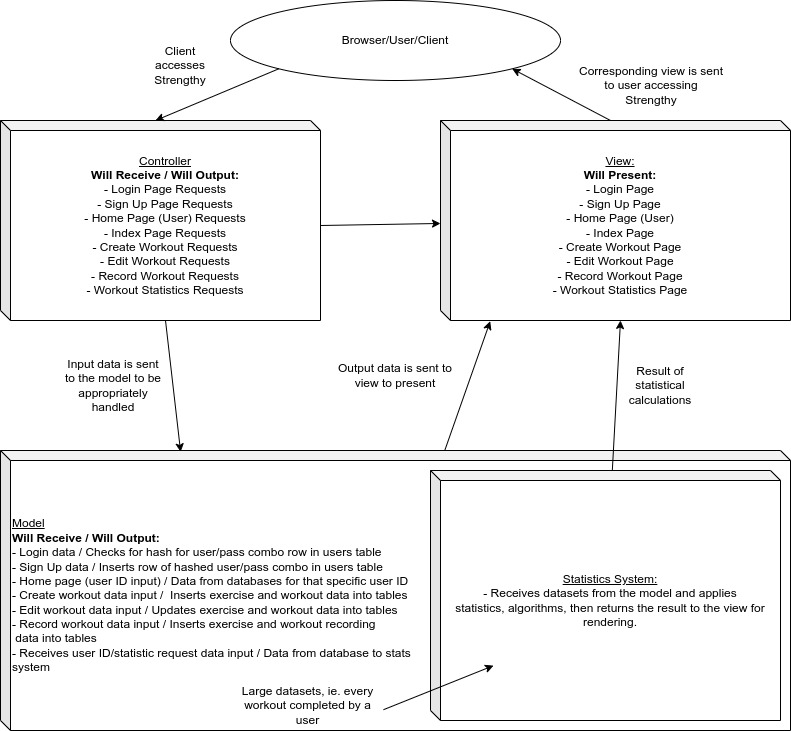
\includegraphics[width=1.0\textwidth]{strengthy_architecture.jpg}
\begingroup
\renewcommand{\section}[2]{}
\begin{thebibliography}{10}
\bigskip
\end{thebibliography}
\endgroup

\section{Implementation}
\subsection{Development Environment and Tools}
\begin{description}
	\item[Environment] For the project, Hayden was developing on Void Linux while Dylan was developing on Arch Linux. Both of our environments typically involved a web browser and the command line.
	\item[Tools] For our tools, we both used the code editor Vim, each with plugins installed to ease development. For source control, we used Git and hosted the source on a VPS. Typically to locally develop and test the web application, we would use the 'flask run' command on the project to start a local instance of the Flask web app.
\end{description}
\subsection{Reused Components}

\section{Testing}
\subsection{Scenarios}
\subsection{Results}

\end{document}
